\documentclass{beamer}
  % Beamer settings
  \usetheme{CambridgeUS}
  \usecolortheme{seagull}
  \usefonttheme{professionalfonts}
  \usefonttheme{serif}

  % Packages and package settings
  \usepackage{fontspec}
    \setmainfont{Charis SIL}
  \usepackage{hyperref}
    \hypersetup{colorlinks=true,
                allcolors=blue}
  \usepackage[backend=biber, style=apa]{biblatex}
    \addbibresource{References.bib}
  \usepackage{graphicx}
    \graphicspath{{./figures/}}
  \usepackage[french]{babel}

  % Document information
  \author{Joshua McNeill}
  \date{28 janvier 2020}
  \title{Exposé de Dewaele (1999)}

\begin{document}
  \begin{frame}
    \titlepage
  \end{frame}

  \begin{frame}{Article}
    \fullcitebib{dewaele_word_1999}
  \end{frame}

  \begin{frame}{Plan}
    \tableofcontents
  \end{frame}

  \AtBeginSection{
    \begin{frame}{Plan}
      \tableofcontents[currentsection]
    \end{frame}
  }

  \section{Introduction}
    % There are a number of interrogative structures
    % Objective: Compare the variation in the use of these structures between native- and non-native speakers
    % Specific research question: "Do advanced speakers of French interlanguage differ from NS in their use of interrogative structures?"
      % If so, do NNSs prefer more formal structures?
    % Expectations: There will be a difference and NNSs will prefer more formal structures
      % Dewaele (1992) found just this for ne deletion among Flemish students

    \begin{frame}{Variables}
      \begin{block}{Deux formes générales}
        \begin{itemize}
          \item Interrogatives totales:
          \item Interrogatives partielles:
        \end{itemize}
      \end{block}
      \begin{columns}
        \column{0.5\linewidth}
          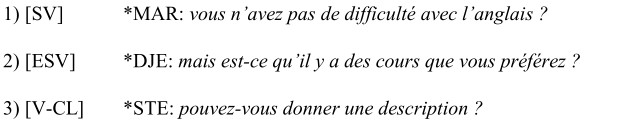
\includegraphics[scale=0.35]{interrogatives_totales.jpg}
        \column{0.5\linewidth}
          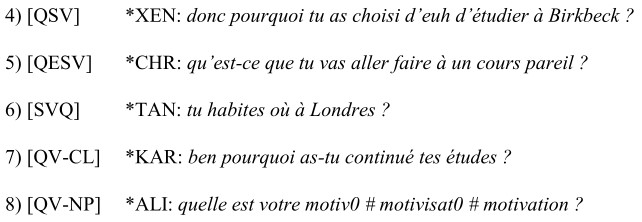
\includegraphics[scale=0.35]{interrogatives_partielles.jpg}
      \end{columns}
    \end{frame}

    % With this many options, there's bound to be variability
      % Coveney (1996) found a range of variation throughout 10 corpora
      % In Quebec
        % Lyster (1996) found preference for inversion (58.4%)
          % Counted -ti structures as inversion: "Je peux-ti t'aider?"
        % Lightbrown (1980) and Lightbrown & d'Anglejean (1985) found the opposite
    % Factors
      % Prescriptive view
        % Wagner & Pinchon (1962) and Grevisse (1980) give four level hierarchy for formality
          % Careful style: [V-CL], [QV-CL], [QV-NP]
            % i.e. inversion
          % Neutral (but inappropriate for writing): [ESV], [QESV]
            % i.e. est-ce que
          % Colloquial: [SV], [SVQ]
          % Working-class (and incorrect): [QSV]
          % Not set in stone: "Pourquoi veux-tu qu'on parte?" is not formal (Huot 1997)
      % Descriptive view
        % Coveney (1996) found several, though the functions of questions in his corpus was far broader
          % Dewaele's questions are essentially limited to requests for info, opinions, and topic introductions
          % Found almost no inversion
          % Pragmatic factors for YNQs
          % Expectation of an answer for ESVs
          % Less informative subjects and verbs yielded more SVGs
          % Men used more QSV than women

    % YNQs are more frequent than WHQs (Gadet 1989; Coveney 1996)
      % Goes on about this for a bit, but it seems beside the point for the actual study

  \section{Methode}
    % Participants (N = 20)
      % Students in the French Department at University of London
      % NS: N = 5; NNS: N = 15
      % 9 women, 11 men
      % 20-60 years old
    % Data gathering
      % Use questionnaires to get biographical data from speakers
        % Gender, age, time spent in France, other languages, profession, etc.
      % Put into pairs and told to interview each other
        % Half mixed and half same gender
        % 2 one hour sessions, switching interviewer every 15 minutes
      % Resulting corpus of 25,068 words

  \section{Resultats}
    \begin{frame}[t]{Comparaison avec d'anciennes études}
      \begin{columns}
        \column{0.5\linewidth}
          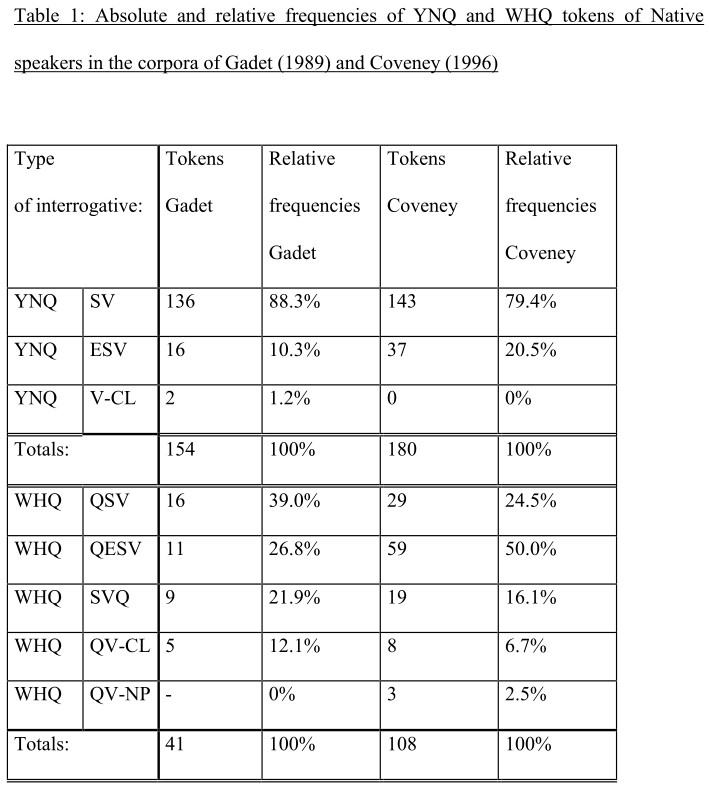
\includegraphics[scale=0.32]{gadet_coveney.jpg}
        \column{0.5\linewidth}
          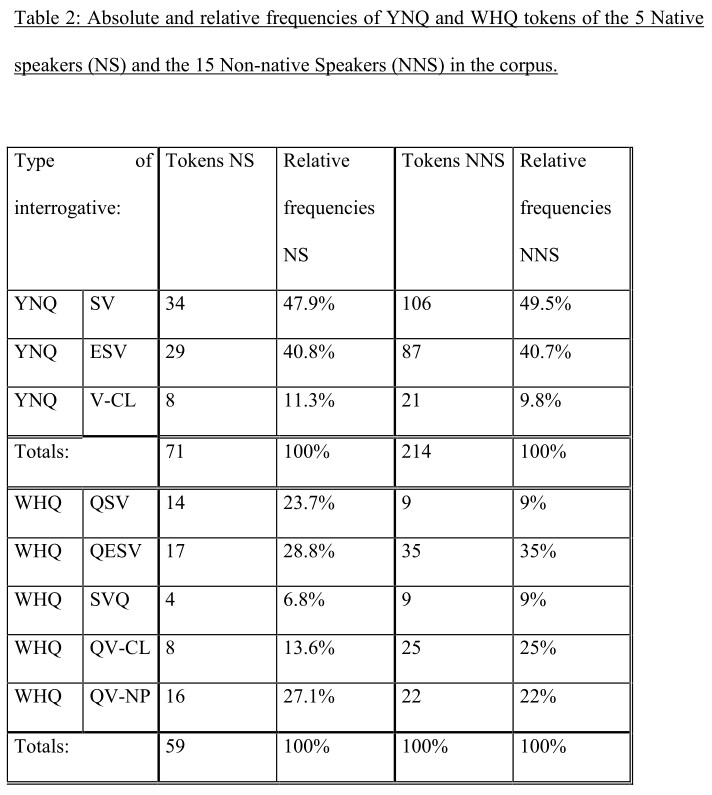
\includegraphics[scale=0.32]{resultats.jpg}
      \end{columns}
    \end{frame}

    \begin{frame}{Pourquoi plus d'inversion?}
      \begin{block}{Une difference de contexte}
        \begin{itemize}
          \item Coveney: A un camp de vacances
          \item Gadet: Des amis sur le téléphone
          \item Dewaele: A une \emph{université}
        \end{itemize}
      \end{block}
    \end{frame}

    \begin{frame}[t]{Facteurs}
      \begin{columns}
        \column{0.5\linewidth}
          \begin{block}{Differences selon les variables biographiques}
            Aucune signification pour:
            \begin{itemize}
              \item l'âge,
              \item le genre,
              \item l'histoire linguistique,
              \item la motivation et
              \item la première langue
            \end{itemize}
            Une signification:
            \begin{itemize}
              \item Locuteurs natifs contre non-natifs pour les interrogatives partielles
            \end{itemize}
          \end{block}
        \column{0.5\linewidth}
          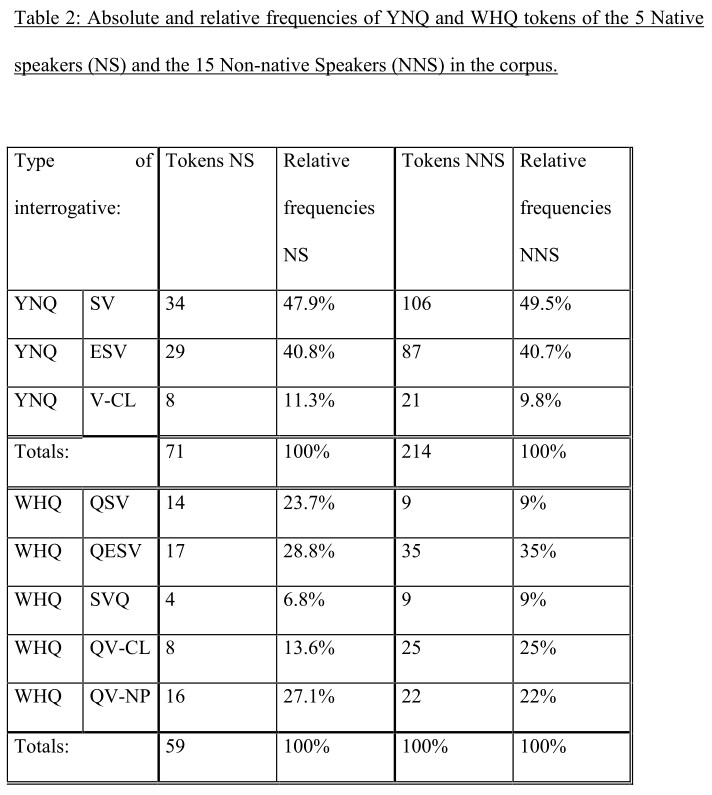
\includegraphics[scale=0.32]{resultats.jpg}
      \end{columns}
    \end{frame}

    \begin{frame}[t]{Facteurs}
      \begin{columns}
        \column{0.47\linewidth}
          \begin{minipage}[t][0.6\textheight]{\linewidth}
            \begin{block}{}
              Différences selon les verbes\phantom{p}
            \end{block}
            \begin{tabular}{l r}
              \emph{Verbe} & \emph{Fréquence d'inversion} \\
              \hline
              avoir        & 23 \\
              pouvoir      & 7 \\
              trouver      & 6 \\
              faire        & 4 \\
              vouloir      & 3
            \end{tabular}
          \end{minipage}
        \column{0.53\linewidth}
          \begin{minipage}[t][0.6\textheight]{\linewidth}
            \begin{block}{}
              Différences selon les temps
            \end{block}
            \begin{tabular}{l r}
              \emph{Temps} & \emph{\% des inversions} \\
              \hline
              Présent      & 78,2 \\
              Passé        & 16,0 \\
              Conditionnel & \\
              ou future    & 5,7
            \end{tabular}
          \end{minipage}
      \end{columns}
      \begin{block}{Mais...}
        On ne connaît pas si cela représente simplement les verbes et les temps les plus fréquents
      \end{block}
    \end{frame}

    \begin{frame}{Facteurs}
      \begin{block}{}
        Presque toutes les inversions [V-CL] et [QV-CL] ont impliqué de nouveaux sujets (95\%)
      \end{block}
      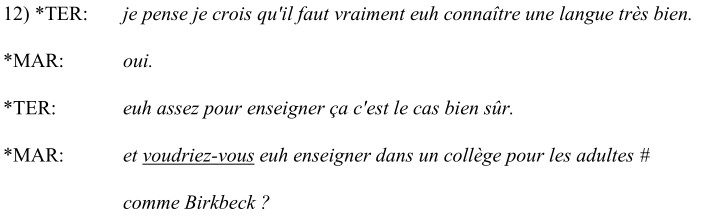
\includegraphics[scale=0.6]{inversion.jpg}
    \end{frame}

    \begin{frame}{Facteurs}
      % Possible influence from English
        % NNSs avoid QSV but not SV
          % Dewaele supposes it has to do with English allowing SV but not QSV
        % NNSs use more QV-CL, familiar from English
    \end{frame}

  \section{Conclusion}
    % The only significant difference between NNSs and NSs was for WHQs
      % NNSs used more formal variants
    % Maybe mention his conclusion that inversions were just generally more common in his corpus
\end{document}
